\documentclass[10pt]{article}
\usepackage[utf8]{inputenc}
\usepackage{pgfplots}
\pgfplotsset{compat=1.15}
\usepackage{mathrsfs}
\usetikzlibrary{arrows}
\pagestyle{empty}
\begin{document}
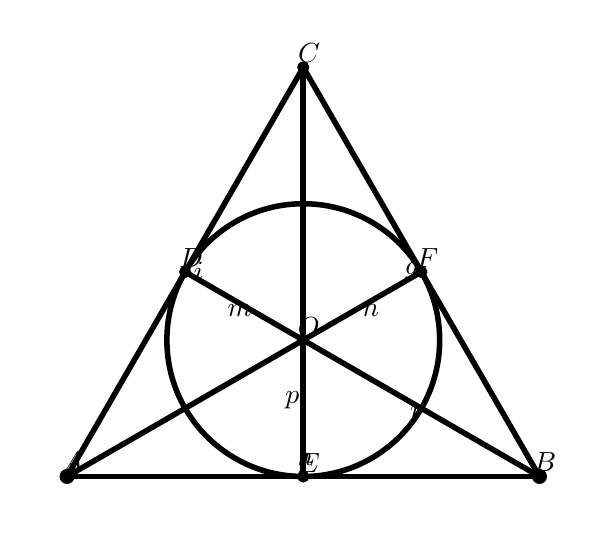
\begin{tikzpicture}[line cap=round,line join=round,>=triangle 45,x=1.0cm,y=1.0cm]
\clip(-3.5,-0.5) rectangle (3.5,5.7);
\draw [line width=2.pt] (-3.,0.)-- (3.,0.);
\draw [line width=2.pt] (0.,5.196152422706632)-- (3.,0.);
\draw [line width=2.pt] (3.,0.)-- (-3.,0.);
\draw [line width=2.pt] (-3.,0.)-- (0.,5.196152422706632);
\draw [line width=2.pt] (0.,1.7320508075688772) circle (1.7320508075688776cm);
\draw [line width=2.pt] (-1.5,2.598076211353316)-- (0.,1.7320508075688772);
\draw [line width=2.pt] (0.,1.7320508075688772)-- (1.5,2.598076211353316);
\draw [line width=2.pt] (0.,1.7320508075688772)-- (0.,0.);
\draw [line width=2.pt] (0.,1.7320508075688772)-- (-3.,0.);
\draw [line width=2.pt] (0.,1.7320508075688772)-- (3.,0.);
\draw [line width=2.pt] (0.,5.196152422706632)-- (0.,1.7320508075688772);
\draw [fill=black] (-3.,0.) circle (2.5pt);
\draw[color=black] (-2.928286390367911,0.18877516105508807) node {$A$};
\draw [fill=black] (3.,0.) circle (2.5pt);
\draw[color=black] (3.071970388249245,0.18877516105508807) node {$B$};
\draw [fill=black] (0.,5.196152422706632) circle (2.0pt);
\draw[color=black] (0.07184199894066727,5.373666035957714) node {$C$};
\draw[color=black] (1.3785181266883058,2.603512645132722) node {$g$};
\draw[color=black] (0.03002836285274284,0.26194902420895577) node {$h$};
\draw[color=black] (-1.3289148100048012,2.603512645132722) node {$i$};
\draw [fill=black] (-1.5,2.598076211353316) circle (2.0pt);
\draw[color=black] (-1.4229954912026312,2.77076718948442) node {$D$};
\draw [fill=black] (1.5,2.598076211353316) circle (2.0pt);
\draw[color=black] (1.5771328981059467,2.77076718948442) node {$F$};
\draw [fill=black] (0.,0.) circle (2.0pt);
\draw[color=black] (0.07184199894066727,0.16786834301112585) node {$E$};
\draw [fill=black] (0.,1.7320508075688772) circle (2.0pt);
\draw[color=black] (0.07184199894066727,1.9031342406599885) node {$O$};
\draw[color=black] (-0.8062443589057459,2.1122024210996106) node {$m$};
\draw[color=black] (0.8558476755892503,2.1122024210996106) node {$n$};
\draw[color=black] (-0.13722618149895488,0.9623274286816895) node {$p$};
\draw[color=black] (1.4412385808201926,0.8159797023739541) node {$r$};
\end{tikzpicture}
\end{document}